\فصل{نتایج آزمایش‌ها}

سه مجموع‌داده استفاده‌شده در این پژوهش توزیع‌های بسیار متفاوتی دارند و برای اهداف متفاوتی مورد استفاده قرار گرفتند. در ادامه نتایج بخش‌های اول و دوم آموزش آورده شده است که در آن به ترتیب طبقه‌بندی‌های بدخیم-خوش‌خیم و طبقه‌بند توموری-سالم آورده شده است.

\section{بخش اول، طبقه‌بند بدخیم و خوش‌خیم} 
دو مجموع‌داده اطلس پاپسوسایتی و ریزآرایه استنفورد برای طبقه‌بندی بدخیم و خوش‌خیم بودن تصاویر نمونه مورد استفاده قرار گرفتند که تعداد کل تصاویر این دو مجموع‌داده روی هم ۱۸۱۰ عدد بوده و از بین آن‌ها به ترتیب ۱۲۵۸، ۱۷۴ و ۳۷۸ تصویر برای آموزش، ارزیابی و تست استفاده شد. بهترین دقتی که بر روی آن‌ها بدست آمد $94.98$ بوده است.
از طرفی، تفاوت فاحشی بین روش‌های مختلف داده‌افزایی و شبکه‌های مختلف دیده نمی‌شود. این اتفاق می‌تواند به دلیل تعداد کم تصاویر آموزش باشد که وجود مجموع‌داده خارجی می‌‌توانست کمک شایانی را به حل این موضوع بکند.
بهترین نتیجه ذکر شده، با روش داده‌افزایی \lr{jit} بدست آمده است. تصاویر موجود در این دو مجموع‌داده، حالت مطالعه موردی\LTRfootnote{Case Study} داشته و از تنوع زیادی در روش رنگ آمیزی شیمیایی سلول‌ها برخوردار بوده است، از این جهت، این روش داده‌افزایی، توانسته تنوع رنگ خوبی در داده‌های آموزش ایجاد کند، تا عملکرد مدل را بهبود ببخشد.
استفاده از گروه داده‌افزایی \lr{base} نیز به نظر تصمیم مناسبی بوده است، زیرا که در بیشتر موارد روش \lr{none} دقت کمتری را نسبت به روش‌های دیگر کسب کرده است.
روش‌ داده‌افزایی \lr{all} از آنجایی که تمام روش‌ها را باهم انجام می‌دهد، به نظر توزیع تصاویر آموزش را بیش از حد تغییر داده، از این جهت، نمودارها، دقت پایداری را نیز در هنگام آموزش نداشته‌اند 
دقت روش \lr{fda} برروی دوره‌ها، در هنگام آموزش بسیار نوسانی بوده است، اما دقت‌های بالایی را در بهترین دوره خود نشان داده است. شاید از این جهت باشد که با جابجایی مولفه‌های پایین فوریه تصاویر، ویژگی‌های مهم از نظر طبقه‌بندی نیز جابجا می‌شوند و معنا و برچسب تصویر نهایی را تغییر می‌دهند.
روش \lr{mixup} نیز به نظر تفاوت چندانی در عملکرد با دیگر روش‌ها نداشته است اما در طی فرآیند آموزش نمودار پایداری را ثبت کرد.
خلاصه از بهترین نتایج کسب شده بر روی مدل‌ها، در جدول \ref{table:papsociety_and_stanford_run_results_summary} آمده است.
\begin{table}[t]
	\caption{نتایج آموزش  با مدل‌های مختلف و روش‌های داده افزایی متفاوت بر روی مجموع دو مجموع‌داده پاپسوسایتی و ریزآرایه بافت استنفورد}
	\centering
	\begin{tabular}{|c|c|c|c|c|}
		\hline
		\rl{معماری شبکه} & \rl{روش‌های داده‌افزایی} & \rl{بهترین دور} & \rl{دقت} & \rl{مساحت زیر نمودار \lr{ROC}} \\
		\hline
		\hline
		\lr{Inception V4} & \lr{none}            & $17$ & $92.94$ & $0.965$ \\
		\lr{Inception V4} & \lr{base \& mixup}   & $85$ & $92.16$ & $0.967$ \\
		\lr{Inception V4} & \lr{base \& fda}     & $85$ & $91.44$ & $0.944$ \\
		\lr{\textbf{Inception V4}} & \lr{\textbf{base \& jit}}     & $58$ & $93.73$ & $0.976$ \\
		\lr{\textbf{Inception V4}} & \lr{\textbf{base \& all}}     & $7$  & $93.88$ & $0.966$ \\
		\lr{Inception V4} & \lr{base-nrs \& jit} & $9$  & $92.69$ & $0.944$ \\
		\lr{Inception V4} & \lr{base-nrs \& all} & $27$ & $94.67$ & $0.943$ \\
		\hline
		\lr{Inception V3} & \lr{none}            & $56$ & $91.25$ & $0.937$ \\
		\lr{\textbf{Inception V3}} & \lr{\textbf{base \& mixup}}   & $81$ & $93.63$ & $0.957$ \\
		\lr{\textbf{Inception V3}} & \lr{\textbf{base \& fda}}     & $99$ & $93.73$ & $0.974$ \\
		\lr{Inception V3} & \lr{base \& jit}     & $2$  & $91.34$ & $0.956$ \\
		\lr{Inception V3} & \lr{base \& all}     & $75$ & $93.41$ & $0.966$ \\
		\lr{Inception V3} & \lr{base-nrs \& jit} & $40$ & $92.06$ & $0.937$ \\
		\lr{Inception V3} & \lr{base-nrs \& all} & $75$ & $93.41$ & $0.966$ \\
		\hline
		\lr{Resnet101}    & \lr{none}            & $14$ & $93.10$ & $0.971$ \\
		\lr{Resnet101}    & \lr{base \& mixup}   & $84$ & $92.22$ & $0.951$ \\
		\lr{\textbf{Resnet101}}   & \lr{\textbf{base \& fda}}     & $40$ & $94.04$ & $0.964$ \\
		\lr{Resnet101}    & \lr{base \& jit}     & $99$ & $92.47$ & $0.947$ \\
		\lr{Resnet101}    & \lr{base \& all}     & $25$ & $92.53$ & $0.962$ \\
		\lr{Resnet101}    & \lr{base-nrs \& jit} & $55$ & $92.28$ & $0.925$ \\
		\lr{Resnet101}    & \lr{base-nrs \& all} & $25$ & $92.53$ & $0.962$ \\
		\hline
		\lr{Resnet18}     & \lr{none}            & $55$ & $89.75$ & $0.922$ \\
		\lr{Resnet18}     & \lr{base \& mixup}   & $7$  & $91.59$ & $0.934$ \\
		\lr{\textbf{Resnet18}}     & \lr{\textbf{base \& fda}}     & $48$ & $94.51$ & $0.943$ \\
		\lr{\textbf{Resnet18}}      & \lr{\textbf{base \& jit}}     & $94$ & $94.98$ & $0.974$ \\
		\lr{Resnet18}     & \lr{base \& all}     & $80$ & $93.88$ & $0.962$ \\
		\lr{Resnet18}     & \lr{base-nrs \& jit} & $90$ & $90.78$ & $0.939$ \\
		\lr{Resnet18}      & \lr{base-nrs \& all} & $13$ & $94.10$ & $0.985$ \\
		\hline
	\end{tabular}
	\label{table:papsociety_and_stanford_run_results}
\end{table}
\begin{table}[t]
	\caption{خلاصه‌ای از نتایج آموزش  با تنظیمات منتخب شده براساس دقت بر روی دو مجموع‌داده پاپسوسایتی و ریزآرایه بافت استنفورد}
	\centering
	\begin{tabular}{|c|c|c|c|c|}
		\hline
		\rl{معماری شبکه} & \rl{روش‌های داده‌افزایی} & \rl{بهترین دور} & \rl{دقت} & \rl{مساحت زیر نمودار \lr{ROC}} \\
		\hline
		\hline
		\lr{\textbf{Inception V4}} & \lr{\textbf{base \& jit}}     & $58$ & $93.73$ & $0.976$ \\
		\lr{\textbf{Inception V4}} & \lr{\textbf{base \& all}}     & $7$  & $93.88$ & $0.966$ \\
		\hline
		\lr{\textbf{Inception V3}} & \lr{\textbf{base \& mixup}}   & $81$ & $93.63$ & $0.957$ \\
		\lr{\textbf{Inception V3}} & \lr{\textbf{base \& fda}}     & $99$ & $93.73$ & $0.974$ \\
		\hline
		\lr{\textbf{Resnet101}}   & \lr{\textbf{base \& fda}}     & $40$ & $94.04$ & $0.964$ \\
		\hline
		\lr{\textbf{Resnet18}}     & \lr{\textbf{base \& fda}}     & $48$ & $94.51$ & $0.943$ \\
		\lr{\textbf{Resnet18}}      & \lr{\textbf{base \& jit}}     & $94$ & $94.98$ & $0.974$ \\
		\hline
	\end{tabular}
	\label{table:papsociety_and_stanford_run_results_summary}
\end{table}

\section{بخش دوم، طبقه‌بند توموری و سالم} 
در قسمت دوم آموزش نیز، مجموع‌داده بزرگ تر دیگری به‌کار رفت. اطلس ژنوم سرطان تیروئید، روی هم‌رفته دارای  ۲۶۵۴۱۸ بریده تصویر است که از بین آن‌ها به ترتیب ۱۸۵۰۹۰، ۲۵۹۰۹ و ۵۴۴۱۹ تصویر برای آموزش، ارزیابی و تست استفاده شد. 
تصاویر بر روی مدل \lr{ResNet101} آموزش داده شدند که مدل توانست وجود یا عدم وجود سلول‌های توموری را در بهترین دوره با دقت  $99.72$ بر روی تصاویر تشخیص دهد.
این مجموع‌داده، اسلاید‌های همگونی داشته که عامل مهمی در عملکرد خوب مدل بوده است.


\begin{figure}
	\begin{center}
		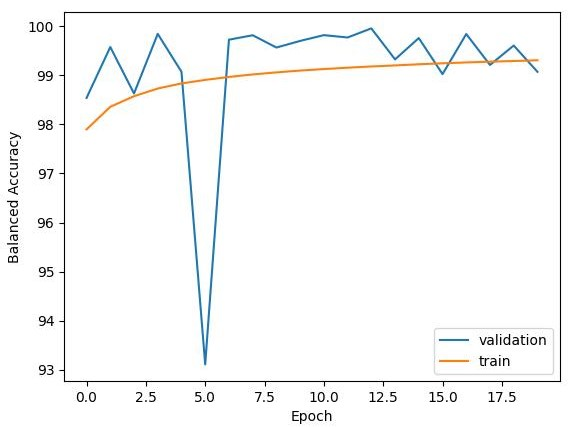
\includegraphics[width=0.8\linewidth]{figs/suggested_methods/val_train_acc_final.jpeg}
	\end{center}
	\caption[ نمودار دقت در هر دوره آموزش مدل بر روی اطلس ژنوم سرطان تیروئید]{بهترین دوره انتخاب شده دوره 12 بوده که دقت و ویژگی عملکرد گیرنده  بر روی داده‌های تست در این دوره به ترتیب $99.72$ و $0.999$ است.}
	\label{nci_dataset_with_resnet101_results}
\end{figure}


\begin{table}[t]
	\caption{خلاصه‌ای از بهترین نتایج کسب شده توسط دو بخش آموزش}
	\centering
	\begin{tabular}{|c|c|c|c|p{0.15\linewidth}|c|c|c|}
		\hline
		\rl{بخش} & \rl{تصاویر آموزش} & \rl{تصاویر ارزیابی} & \rl{تصاویر تست} & \rl{برچسب} & \rl{دوره} & \rl{دقت} & \rl{AUC}
		\\
		\hline
		\hline
		\rl{بخش اول} & \rl{۱۲۵۸} & \rl{۱۷۴} & \rl{۳۷۸} & \rl{خوش‌خیم} \newline \rl{بدخیم}& \rl{۹۴} & \rl{$94.98$} & \rl{$0.974$}\\
		\hline
		\hline
		\rl{بخش دوم} & \rl{۱۸۵۰۹۰} & \rl{۲۵۹۹۰۹} & \rl{۵۴۴۱۹} & \rl{سالم}\newline \rl{توموری} & \rl{۱۲} & \rl{$99.72$} & \rl{$0.999$}\\ 
		\hline
	\end{tabular}
	\label{table:section_results_and_details}
\end{table}


